\section{BTB-X}
\label{cal:sec:design}


To reduce the overall storage cost, this work seeks to minimize the storage requirements of the costliest fields making up each BTB entry, i.e. target and tag, through two ideas: partitioning and hashing.  

\begin{figure}[t!]
    \centering
    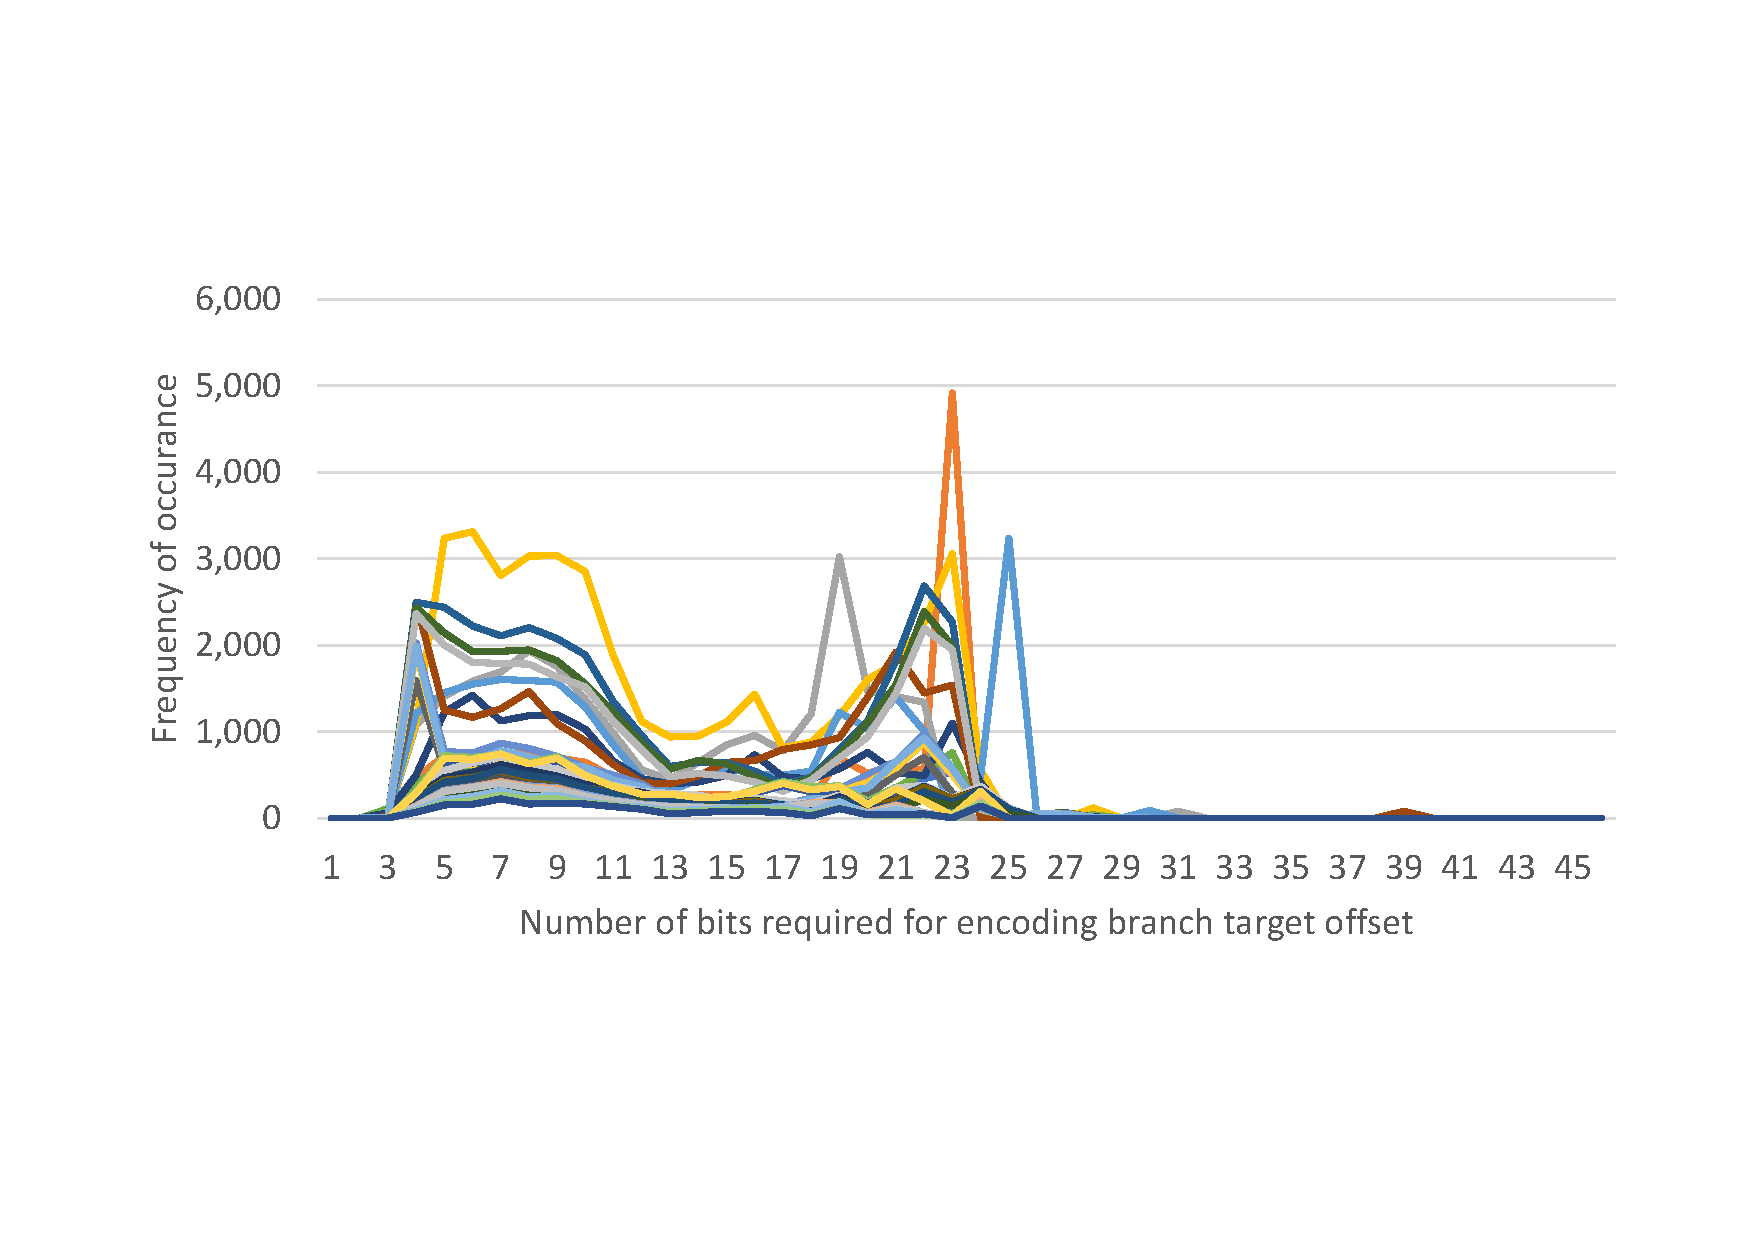
\includegraphics[width=\columnwidth, trim=60 140 60 155, clip]{figures/OffsetLen1.pdf}
    \caption{Distribution of branch target offsets.}
    \vspace{-0.1in}
    \label{cal:fig:offsets}
\end{figure}

\subsection{Partitioned BTB}

As \Cref{cal:fig:conv-btb} shows, the largest contributor to storage cost is the target field, which stores the branch target address. For instance, in the ARM v8 ISA, which uses a 32-bit fixed length instruction encoding, the target address is 46 bits long with a 48-bit virtual address space. Our key insight is that targets of most branches lie relatively close in the virtual address space to the branch itself. As a result, encoding the {\em distance} to the target, in the form of an offset from the branch instruction, instead of a full target address, can provides drastic storage savings. 

\Cref{cal:fig:offsets} plots the distribution of offsets in the branch working sets of our workload traces. Offsets are calculated in instruction words, which are 32 bits in the ARM v8 ISA. The data includes both conditional and unconditional branches; hence, it comprehensively covers the full branch working set. The X-axis shows the number of bits required to encode the offset, while the Y-axis plots the frequency of occurrence. Note that, in addition to bits for encoding the offset, an additional bit is required for the direction of the offset (forward/backward). 

As the figure shows, short offsets dominate the distribution with 37\% of branches requiring only seven bits or fewer for their offsets. A further 30\% of branches only require between 8 and 14-bits to represent their offsets. The reason why such a high fraction of offsets is short is that conditional branches dominate the dynamic branch working set, and they tend to have short offsets~\cite{boomerang}. This is because conditional branches generally guide the control flow only inside a function; meanwhile, software engineering principles favor small functions, thus restricting conditional branch offsets to short distances.

Perhaps surprisingly, \Cref{cal:fig:offsets} also shows that very few branches require a large number of bits to encode their offset. Indeed, a meagre 1\% of branches requires 25 bits or more for their offset encoding. The sum of these results indicates that reserving space for the full 46-bit target address results in an appalling under-utilization of BTB storage, since 99\% of branches need at most half the number of bits needed to represent the full target address if offsets are used instead.  

Based on these insights, we propose to partition a single logical BTB into multiple physically-separate BTBs. The BTBs differ amongst themselves only in the size of the offset. When the branch prediction unit queries an address, all BTB partitions are accessed in parallel, hence presenting a logical equivalent of a monolithic BTB. If the core queries the BTB with $n$ addresses per cycles, each BTB-X partition must be accessed with all $n$ addresses.

\begin{figure}
    \centering
    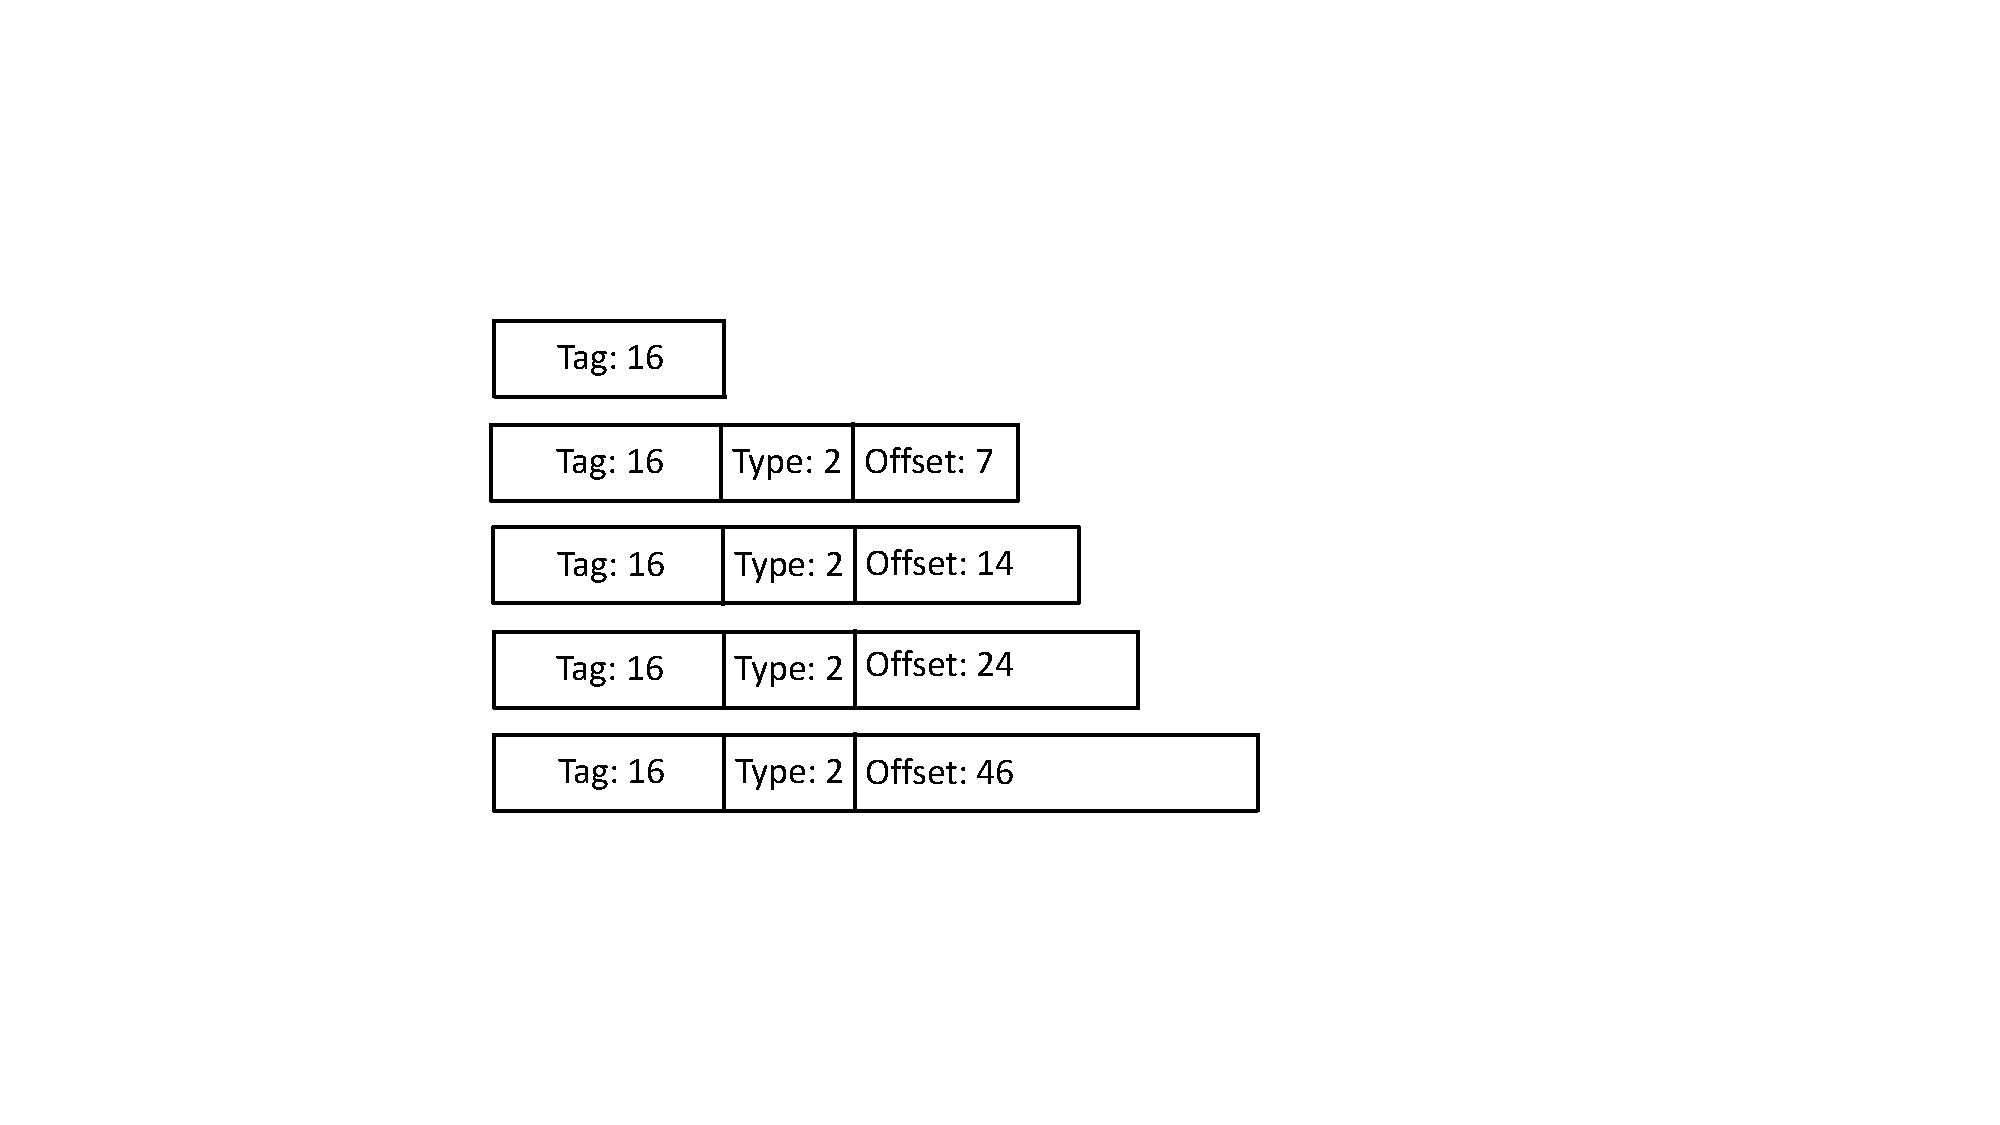
\includegraphics[width=0.7\columnwidth, trim=230 150 340 150, clip]{figures/x-btb.pdf}
    \caption{BTB entry composition for BTB-X partitions.} 
    \label{cal:fig:btb-dist}
    \vspace{-0.1in}
\end{figure}

\Cref{cal:fig:btb-dist} shows the BTB partitions used by our proposed BTB organization, called BTB-X.
It uses five different BTBs with offset field sizes of 0, 7, 14, 24 and 46 bits. The BTB with no offset field (i.e., 0-bit offset) tracks only return instructions. Recall from \Cref{cal:sec:background} that return instructions read their target address from RAS; as such, there is no need to allocate space for targets of returns in the BTB. Further, as all instructions in this BTB are returns, it does not require the branch \textit{type} field either. Other branches are allocated entries in one of the remaining  four BTBs based on the minimum number of bits required to encode their offsets. For example, if a branch requires 10 bits for encoding its target offset, it is allocated an entry in the BTB with target offset field size of 14 bits.

We further make use of the data in \Cref{cal:fig:offsets} to size each of the BTBs. Because very few branches require more than 24 bits to encode their target offsets, the BTB with the 46-bit offset field is allocated the fewest entries. Meanwhile, the BTBs corresponding to 7-, 14-, and 24-bit offset are allocated a similar number of entries, as the frequency of 1-7 bit, 8-14 bit, and 15-24 bit offsets is about same -- 37\%, 30\% and 32\% respectively.

\subsection{Tag Compression}

Tags comprise the second largest source of storage overhead in each BTB entry, requiring 39 bits in the baseline design.
To further reduce the storage requirement, BTB-X uses a compressed 16-bit tag in all of its BTBs. Our compression scheme maintains the 8 low-order bits same as in the full tag. The remaining bits of the full tag are folded, using the XOR operator, in blocks of eight to compute the 8 higher-order bits for the compressed tag. As our evaluation shows, the performance impact of this scheme is negligible as the hashing function (folded XOR) preserves most of the entropy found in the high-order bits.

\subsection{Applicability to Basic-Block-Based BTBs}
While this work describes BTB-X in the context of an instruction-based BTB organization (i.e., the BTB is accessed using individual instruction addresses), our insights and design are equally applicable to basic-block-based BTBs (BB-BTBs)~\cite{fdip, boomerang, shotgun}. BB-BTBs are similar to instruction-based ones but are accessed using a basic-block address. Because existing BB-BTB designs store full branch targets and offsets, they would benefit from optimizations described in this work.
